\documentclass[12pt, a4paper]{article}



%\usepackage[cp1251]{inputenc}
\usepackage{a4wide} % уменьшает поля
\textwidth=11.5cm

\usepackage[utf8]{inputenc}
\usepackage[russian]{babel} % включает русский язык
\usepackage{graphicx} % позволяет подключить .eps - файлы
\usepackage{amsmath}
\usepackage{amsthm} % теоремы от AMS
\usepackage{amssymb} % для работы с математическими R и проч.
\usepackage{floatrow}
\usepackage{mathrsfs}
\usepackage{mathtools} % содержит \coloneqq -- присванивание

\usepackage{accents}
\newcommand{\ubar}[1]{\underaccent{\bar}{#1}}

\usepackage[usenames]{color} % чтобы цвета в hyperref понимались
\usepackage{ulem} % дает зачеркнутый текст по \sout
\usepackage[unicode,
			breaklinks,colorlinks,
			linkcolor=Black,
			citecolor=Black,
			hyperfootnotes=false]
			{hyperref} % кликабельное оглавление без кликабельных футноутов


\newtheoremstyle{rusdef}
  {3pt}% measure of space to leave above the theorem. E.g.: 3pt
  {3pt}% measure of space to leave below the theorem. E.g.: 3pt
  {\itshape}% name of font to use in the body of the theorem
  {\parindent}% measure of space to indent
  {\bfseries}% name of head font
  {.}%
  {.5em}%
  {}
   

\theoremstyle{rusdef}
\newtheorem{define}{Определение} % определение по-русски
\newtheorem{theorem}{Теорема}
\newtheorem{prop}{Предложение}
\renewcommand\qedsymbol{$\blacksquare$}
\newtheorem{statement}{Утверждение}
\newtheorem{remark}{Замечание}
\newtheorem{lemma}{Лемма}
\newtheorem{corol}{Следствие}
\newtheorem{assume}{Предположение}
\newtheorem{example}{Пример}

\newcommand\abs[1]{\left\lvert #1 \right\rvert} % модуль
\newcommand\bracket[1]{\left( #1 \right)} % скобки
\newcommand\scalar[1]{\left < #1 \right >} % скалярное произведение
\newcommand{\R}{\ensuremath{\mathbb{R}}} % R - мн-во вещественных чисел
\newcommand{\N}{\ensuremath{\mathbb{N}}} % N - мн-во натуральных чисел
\newcommand{\X}{\mathscr{X}} % красивая Х для начального и конечного множеств
\renewcommand{\P}{\mathscr{P}} % красивая P для ограничений на управление
\newcommand{\then}{\Rightarrow}
\newcommand{\h}{\mathbb{h}}
\newcommand{\e}{\mathbf{e}}

\renewcommand{\H}{\mathcal{H}} % красивая H для Гамильтона-Понтрягина
\newcommand{\M}{\mathcal{M}} % красивая M для Максимума
\renewcommand{\L}{\mathscr{L}} % красивая L для Лагранжа
\renewcommand{\d}{\partial} % чтобы долго не писать частную производную
\newcommand{\norm}[1]{\left\lVert #1 \right\rVert} % норма
\DeclareMathOperator*{\thus}{\Rightarrow} % следствие с возможностью использовать limits
\DeclareMathOperator*{\To}{\longrightarrow}
\DeclareMathOperator*{\Argmax}{Argmax} % Argmax с возмножностью использовать limits

\usepackage{indentfirst} % абзац после заголовка

\DeclareMathOperator{\sgn}{sgn} % сигнум
\DeclareMathOperator{\rank}{rank} % ранг

\begin{document}

\begin{center}
{\Huge \textbf{Обобщение принципа максимума}}
\end{center}

\begin{equation}
\dot{x}(t) = f(t, x(t), u(t)), \;\; u(t) \in \P(t)
\end{equation}
Обозначим
$$
e = (t_0, x^0, t_1, x^1) \in \R \times \R^n \times \R \times \R^n
$$
и рассмотрим множество
$$
E = \left\{ e \colon \exists u(\cdot) \colon x(t_1, t_0, x^0 \rvert u(\cdot)) = x^1 \right\},
$$
т.~е. множество всех таких четвёрок $(t_0, x^0, t_1, x^1)$, что систему (1) можно перевести из $x(t_0) = x^0$ в $x(t_1) = x^1$.

Рассмотрим функции
$$
\varphi_j \in C^1 \left(\R \times \R^n \times \R \times \R^n \to \R \right), \;\;\; j = 0, 1, \ldots, k,
$$
задача оптимизации с ограничениями типа <<равенство>>:
\begin{equation}\label{eq:opt_problem}\tag{\text{ЗО}}
\varphi_0(e) \to \inf\limits_{u(\cdot)}
\end{equation}
при
$$
E^0 = \left\{ e \in E \colon \varphi_1(e) = \ldots = \varphi_k(e) = 0 \right\}.
$$

\begin{theorem}
Пусть $\left\{ x^*(\cdot), u^*(\cdot) \right\}$ определены $e^* \in E$ такие, что $e^* = (t_0^*, x^{0*}, t_1^*, x^{1*})$ --- решение \eqref{eq:opt_problem} $\thus$ \\
$\exists \bar{\lambda} = (\lambda_0, \lambda_1, \ldots, \lambda_k) \in \R^{k+1}$, $\bar{\lambda} \neq \theta, \lambda_0 \leqslant 0$, $\exists \psi^* \colon [t_0^*, t_1^*] \to \R^n$,\\
$\H(t,x,\psi,u) = \scalar{\psi, f(t,x,u)}$, $\M(t,x,\psi) = \sup\limits_{u \in \P} \H(t,x,\psi,u)$:

\begin{enumerate}
\item Сопряжённая система
\begin{equation}\tag{\text{СС}}
\dfrac{d\psi^*}{dt} = -\dfrac{\d \H}{\d x}
_{\left|
\begin{matrix}
x = x^*(t)\\ u = u^*(t) \\ \psi = \psi^*(t)
\end{matrix}
\right.}
\end{equation}

\item Условие максимума
\begin{equation}\tag{\text{УМ}}
\H(t, x^*(t), \psi^*(t), u^*(t)) = \sup\limits_{u \in \P} \H(t, x^*(t), \psi^*(t), u) =
\end{equation}
$$
= \M(t, x^*(t), \psi^*(t))
$$

\item Условия трансверсальности (!)
\begin{equation}\tag{\text{УТ}}
\begin{aligned}
& \psi^*(t_1^*) = \left[ \dfrac{\d \bar{\Phi}(e^*)}{\d x^1} \right]^T \bar{\lambda}, \\
& \psi^*(t_0^*) = - \left[ \dfrac{\d \bar{\Phi}(e^*)}{\d x^0} \right]^T \bar{\lambda},
\end{aligned}
\end{equation}
$$
\H(t_1^*, x^{1*}, \psi^*(t_1^*), u^*(t_1^*)) = - \left[ \dfrac{\d \bar{\Phi}(e^*)}{\d t_1} \right]^T \bar{\lambda},
$$
$$
\H(t_0^*, x^{0*}, \psi^*(t_0^*), u^*(t_0^*)) = \left[ \dfrac{\d \bar{\Phi}(e^*)}{\d t_0} \right]^T \bar{\lambda},
$$
где $\bar{\Phi} = (\varphi_0, \varphi_1, \ldots, \varphi_k)^T$.

\item Если $\dfrac{\d f}{\d t} \in C$, тогда
$$
\exists \dfrac{d \H(t, x^*(t), \psi^*(t), u^*(t))}{dt} = \left\{ \text{п.в. t} \right\} =
$$
$$
= \dfrac{d \M(t, x^*(t), \psi^*(t))}{dt} = \scalar{\psi^*(t), \dfrac{\d f}{\d t}}.
$$
\end{enumerate}
\end{theorem}

Как это связано с нашей формулировкой ПМП?

Условие нетривиальности автоматически выполняется, т.~к. из $\bar{\lambda} \neq 0$ и 3) $\thus$ \\ $\psi \not\equiv 0 \thus \psi \neq 0$.
$$
\L = \lambda_0\varphi_0(e) + \lambda_1\varphi_1(e) + \ldots + \lambda_k\varphi_k(e) = \scalar{\bar{\lambda}, \bar{\Phi}},
$$
$$
\Delta\L = \scalar{\bar{\lambda}, \bar{\Phi}(t_0, x^0, t_1, x^1 + \delta x^1) - \bar{\Phi}(t_0, x^0, t_1, x^1)} =
$$
$$
= \scalar{\bar{\lambda}, \dfrac{\d \bar{\Phi}}{\d x^1} \Delta x^1} + \bar{o}(\norm{\Delta x^1}) = \scalar{ \left[\dfrac{\d \bar{\Phi}}{\d x^1}\right]^T \bar{\lambda}, \Delta x^1} + \bar{o}(\norm{\Delta x^1}).
$$

Поэтому $\left[\dfrac{\d \bar{\Phi}(e^*)}{\d x^1}\right]^T \bar{\lambda} = \dfrac{\d \L}{\d x^1}$. Аналогично,
$$
-\left[\dfrac{\d \bar{\Phi}(e^*)}{\d x^0}\right]^T \bar{\lambda} = \dfrac{\d \L}{\d x^0},
$$
$$
-\left[\dfrac{\d \bar{\Phi}(e^*)}{\d t_1}\right]^T \bar{\lambda} = \dfrac{\d \L}{\d t_1},
$$
$$
\left[\dfrac{\d \bar{\Phi}(e^*)}{\d t_0}\right]^T \bar{\lambda} = \dfrac{\d \L}{\d t_0}.
$$

Вспомним одну из рассмотренных ранее формулировок:
$\hat{t}_0$ --- фикс., $t_1$ --- своб., $x^0 \in \X^0$, $x^1 \in \X^1$,
$$
\mathcal{J} = \int\limits_{t_0}^{t_1} f^0(t, x(t), u(t)) dt \to \inf\limits_{u(\cdot)}.
$$
$$
x^0 \in \X^0 \Leftrightarrow g^0(x^0) = \left[\begin{matrix} g_1^0(x^0)\\ \ldots \\ g_{d_0}^0 (x^0) \end{matrix}\right] = 0;
$$
$$
x^1 \in \X^1 \Leftrightarrow g^1(x^1) = \left[\begin{matrix} g_1^1(x^1)\\ \ldots \\ g_{d_1}^0 (x^1) \end{matrix}\right] = 0.
$$

Пусть $\bar{x} = (x_0, x_1, \ldots, x_n)^T$.
$$
\left\{
\begin{aligned}
& \dot{x}_0 = f^0(t,x,u), \\
& \dot{x}_1 = f^1(t,x,u), \\
& \ldots \\
& \dot{x}_n = f^n(t,x,u), \\
& x_0(t_0) = 0, \\
& \mathcal{J} = x_0(t_1) \to \inf\limits_{u(\cdot)}.
\end{aligned}
\right.
$$

Далее рассмотрим автономный случай.
$$
\begin{aligned}
& \hspace*{0.9cm} \dot{\bar{x}} = \bar{f}(\bar{x}, u), \;\; e = (t_0, \bar{x}^0, t_1, \bar{x}^1)\\
& \hspace*{0.9cm} \varphi_0 = x_0^1\\
& \hspace*{0.9cm} \varphi_1 = t_0 - \hat{t}_0 \;\;  (\text{= 0, а на $t_1$ ограничений нет})\\
& \hspace*{0.9cm} \varphi_2 = x_0^0 \;\; (= 0)\\
& d_0 \left\{
\begin{aligned}
& \varphi_3 = g_1^0(x^0) \;\; (= 0) \\
& \ldots\\
& \varphi_{d_0 + 2} = g_{d_0}^0(x^0) \;\; (=0)\\
\end{aligned}
\right.\\
& d_1 \left\{
\begin{aligned}
& \varphi_{d_0 + 3} = g_1^1(x^1) \;\; (= 0) \\
& \ldots\\
& \varphi_{d_0 + d_1 + 2} = g_{d_1}^1(x^1) \;\; (=0)
\end{aligned}
\right.
\end{aligned}
$$

$$
\bar{\psi}^* \colon \;\; \text{(СС), (УМ)}; \;\; \H = \psi_0 f^0 + \scalar{\psi, f},
$$
$$
\bar{\psi}^*(t_1^*) = \left[ \begin{matrix}
\lambda_0,\\ \left( \dfrac{\d g^1}{\d x^1} \right)^T \left[ \begin{matrix}
\lambda_{d_0 + 3} \\ \ldots \\ \lambda_{d_0 + d_1 + 2}
\end{matrix} \right]
\end{matrix} \right],
$$
т.~е.
$$
\begin{matrix}
& \psi_0^*(t_1^*) = \lambda_0, \\
& \psi_i^*(t_1^*) = \scalar{\dfrac{\d g^1}{\d x^1_i}, \left[ \begin{matrix}
\lambda_{d_0 + 3}\\ \ldots \\ \lambda_{d_0 + d_1 + 2}
\end{matrix} \right]}, i = 1, \ldots, n.
\end{matrix}
$$

$$
\bar{\psi}^*(t_0^*) = - \left[ \begin{matrix}
\lambda_2,\\ \left( \dfrac{\d g^0}{\d x^0} \right)^T \left[ \begin{matrix}
\lambda_{3} \\ \ldots \\ \lambda_{d_0 + 2}
\end{matrix} \right]
\end{matrix} \right],
$$
т.~е. ...

Здесь 
$$
\dfrac{\d g^0}{\d x^0} = \left[ \begin{matrix}
&\dfrac{\d g_1^0}{\d x_1^0} &\ldots &\dfrac{\d g_1^0}{\d x_n^0}\\
&\vdots &\ddots &\vdots\\
&\dfrac{\d g^0_{d_0}}{\d x_1^0} &\ldots &\dfrac{\d g^0_{d_0}}{\d x_n^0}
\end{matrix} \right] \in \R^{d_0 \times n}
$$

$\dot{\psi}_0 = 0 \thus \psi_0 \equiv \mathrm{const} = \lambda_0 = -\lambda_2$ (тут $\lambda_0 \leqslant 0$).

$$
\left(\dfrac{\d g^0}{\d x^0}\right)^T = \left[ \begin{matrix}
&\dfrac{\d g_1^0}{\d x_1^0} &\ldots &\dfrac{\d g^0_{d_0}}{\d x_1^0}\\
&\vdots &\ddots &\vdots\\
&\dfrac{\d g_1^0}{\d x_n^0} &\ldots &\dfrac{\d g^0_{d_0}}{\d x_n^0}
\end{matrix} \right];
$$
$T_{x^0} \X^0 = \ker \dfrac{\d g^0}{\d x^0}, \;\;\; \mathrm{im} \left(\dfrac{\d g^0}{\d x^0}\right)^T = \left( \ker \dfrac{\d g^0}{\d x^0} \right)^{\bot}$.

Тем самым, $\psi^*(t_0^*) \bot T_{x^{0*}} \X^0$.

УТ по времени:
$$
\left. \H \right|_{t = t_1^*} = -0 \thus \left\{ \M \equiv \mathrm{const}, \; \left. \M \right|_{t = t_1^*} = 0 \right\} \thus \M \equiv 0.
$$
$$
\left. \H \right|_{t = t_0^*} = \lambda_1 \text{ --- лишнее}
$$

Пусть теперь $\hat{t}_0$ --- фикс., $\hat{t}_1$ --- фикс., $\hat{x}^0$ --- нач. точка, $\hat{x}^1$ --- кон. точка.

Подготовка УТ:
$$
\begin{aligned}
& \varphi_0 = x^1_0\\
& \varphi_1 = t_0 - \hat{t}_0\\
& \varphi_2 = t_1 - \hat{t}_1\\
& \varphi_3 = x^0_0\\
& \left[ \begin{matrix}\varphi_4 \\ \vdots \\ \varphi_{n+3} \end{matrix} \right] = x^0 - \hat{x}^0 \;\;\;\;\; (\varphi_{3+i} = x^0_i - \hat{x}^0_i, i = 1, \ldots, n)\\
& \left[ \begin{matrix}\varphi_{n+4} \\ \vdots \\ \varphi_{2n+3} \end{matrix} \right] = x^1 - \hat{x}^1 \;\;\;\;\; (\varphi_{n+3+i} = x^1_i - \hat{x}^1_i, i = 1, \ldots, n)
\end{aligned}
$$

Тогда УТ:
$$
\bar{\psi}^*(t^*_1) = \left[ \begin{matrix}
\lambda_0 \\ \lambda_{n+4} \\ \vdots \\ \lambda_{2n+3}
\end{matrix} \right], 
\;\;\;\;\;\;\;
\bar{\psi}^*(t^*_0) = - \left[ \begin{matrix}
\lambda_3 \\ \lambda_{4} \\ \vdots \\ \lambda_{n+3}
\end{matrix} \right]
$$
При этом
$$
\H |_{t=t^*_1} = -\lambda_2, \;\;\;\;\; \H |_{t = t^*_0} = \lambda_1,
$$
$$
\psi^*_0 \equiv \mathrm{const} = \lambda_0 = -\lambda_3, \;\;\; \M \equiv \mathrm{const}
$$
Остальные УТ никакой информации не дают $\thus$ они нам и не нужны.

\subsection*{Задача со свободным правым концом}
$$
\left\{
\begin{aligned}
& \dot{x} = f(t, x, u), \\
& x(t_0) = x^0,
\end{aligned}
\right.
$$
$t_0, x^0, t_1$ --- фиксированы,
$$
\mathcal{J} = \int\limits_{t_0}^{t_1} f^0(x(t), u(t)) dt + \phi(x(t_1)) \to \inf\limits_{u(\cdot)}
$$

Переобозначим: $\hat{x}^0, \hat{t}_0, \hat{t}_1$.
$$
\begin{aligned}
& \varphi_0 = x^1_0 + \phi(x^1) \\
& \varphi_1 = t_0 - \hat{t}_0 \\
& \varphi_2 = t_1 - \hat{t}_1 \\
& \varphi_3 = x^0_0 \\
& \varphi_4 = x^0_1 - \hat{x}^0_1 \\
& \ldots \\
& \varphi_{n+3} = x^0_n - \hat{x}^0_n
\end{aligned}
$$

ПМП утверждает, что $\exists \bar{\psi}^* \colon [t^*_0, t^*_1] \to \R^{n+1}$:
\begin{enumerate}
\item (СС) $\dfrac{d\psi}{dt} = \left. -\dfrac{\d \H}{\d x} \right|_{...}$
\item (УМ)
\item (УТ) $\bar{\psi}^*(t^*_1) = \left[ \begin{matrix} \lambda_0 \\ \lambda_0 \dfrac{\d \phi}{\d x} \end{matrix} \right]$\\
		   $\bar{\psi}^*(t^*_0) = \left[ \begin{matrix} \lambda_3 \\ \lambda_4 \\ \vdots \\ \lambda_{n+3} \end{matrix} \right]$\\
		   $\H |_{t = t^*_1} = -\lambda_2; \;\;\; \H _{t = t^*_0} = \lambda_1$
\end{enumerate}

Второе у третье условия из (УТ) не дают нам никакой информации. Из первого же следует, что
$$
\psi^*_0 \equiv \mathrm{const} = \lambda_0 \leqslant 0 \thus \lambda_0 < 0
$$
(иначе нарушится условие нетривиальности $\bar{\lambda} \neq 0$).
Возьмём $\lambda_0 = -1$ и перепишем:

3') $\psi^*_0 \equiv -1, \;\;\;\;\; \psi^*(t^*_1) = -\dfrac{\d \phi}{\d x}$.

Докажем полученную формулировку 1), 2), 3') ПМП для задачи со свободным правым концом.
\begin{proof}
Пусть $\left\{ x^*(\cdot), u^*(\cdot) \right\}$ --- оптимальная пара. $\psi^*_0 := -1$;
$$
\psi^*(t) := -\dfrac{\d \phi(x^*(t_1^*))}{\d x} +
$$
$$
+ \int\limits_{t_1}^{t} \left( -\psi^*_0 \dfrac{\d f^0(x^*(s), u^*(s))}{\d x} - \left( \dfrac{\d f}{\d x}(x^*(s), u^*(s)) \right)^T \psi^*(s) \right) ds
$$

$$
\left\{
\begin{aligned}
& \dfrac{d \psi^*(t)}{dt} = \dfrac{\d f^0}{\d x}(x^*(t), u^*(t)) - \left( \dfrac{\d f}{\d x} \right)^T \psi^*(t), \\
& \psi^*(t_1) = - \dfrac{\d \psi(x^*(t_1))}{\d x}.
\end{aligned}
\right.
$$

Осталось доказать (УМ):
$$
- f^0 (x^*(t), u^*(t)) + \scalar{\psi^*(t), f(x^*(t), u^*(t))} \geqslant
$$
$$
\geqslant -f^0 (x^*(t), v) + \scalar{\psi^*(t), f(x^*(t), v))}
$$
для всех $\forall v \in \P$ ($v$ --- конечномерный вектор).

$$
J[u(\cdot)] = \int\limits_{t_0}^{t_1} f^0(x(t), u(t)) dt + \phi(x(t_1)) \geqslant J[u^*(\cdot)],
$$
$$
\forall u(\cdot) \in U_{\varepsilon}(u^*(\cdot))
$$

В каком смысле нам здесь понимать $\varepsilon$-окрестность?

Пусть  $u^*(\cdot)$ --- кусочно-непрерывна и непрерывна слева, тогда в качестве вариации $u$ можем рассмотреть \textbf{игольчатую вариацию} следующего вида:\\
$t_0 < \tau \leqslant t_1, \; 0 < \varepsilon \leqslant \tau - t_0, \;\; v \in \P$

\begin{figure}[h!]
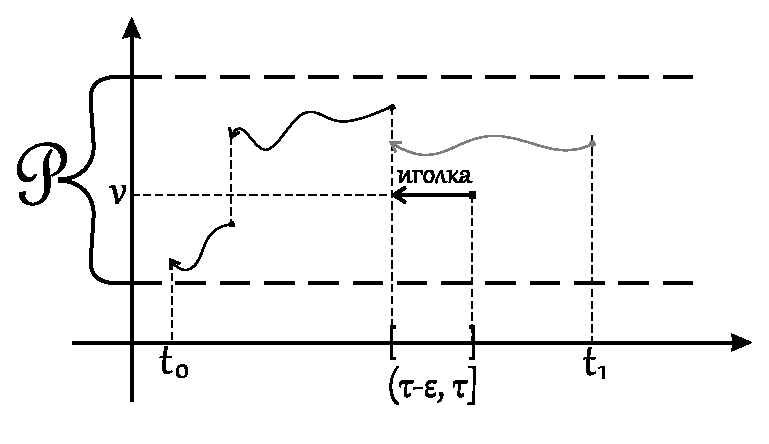
\includegraphics[scale=0.7]{niddle.eps}
\end{figure}

$$
u_{\varepsilon}(t) = 
\left\{
\begin{aligned}
& u^*(t), & t \in [t_0, t_1] \setminus (\tau - \varepsilon, \tau]  \\
& v, & t \in (\tau - \varepsilon, \tau]
\end{aligned}
\right.
$$

Итак, $J[u_{\varepsilon}(t)] \geqslant J[u^*(\cdot)] \thus \left\{ \varepsilon > 0 \right\} \thus$
$$
\thus \dfrac{J[u_{\varepsilon}(\cdot)] - J[u^*(\cdot)]}{\varepsilon} \geqslant 0 \thus
$$
$$
\thus \liminf\limits_{\varepsilon \to +0} \dfrac{J[u_{\varepsilon}(\cdot)] - J[u^*(\cdot)]}{\varepsilon} \geqslant 0
$$

\begin{lemma}
$x_{\varepsilon}(t) = x^*(t) + \varepsilon\delta x(t) + \bar{o}(\varepsilon)$, где
$$
\left\{
\begin{aligned}
& \dfrac{d}{dt} \left( \delta x(t) \right) = \left( \dfrac{\d f(x^*(t), u^*(t))}{\d x} \right) \delta x(t), \;\;\; t \geqslant \tau, \\
& \delta x(\tau) = f(x^*(\tau), v) - f(x^*(\tau), u^*(\tau)),
\end{aligned}
\right.
$$
при $t < \tau$ выполняется $\delta x(t) = 0$, то есть $x_{\varepsilon}(t) = x^*(t), \;\; t < \tau$ и при $t \geqslant \tau$
$$
\dfrac{x_{\varepsilon}(t) - x^*(t)}{\varepsilon} \To\limits_{\varepsilon \to +0} \delta x(t).
$$
\end{lemma}
\begin{proof}[Доказательство леммы]
$$x^*(t) = x^0 + \int\limits_{t_0}^{t} f(x^*(s), u^*(s)) ds$$
$$x_{\varepsilon}(t) = x^0 + \int\limits_{t_0}^{t} f(x_{\varepsilon}(s), u_{\varepsilon}(s)) ds$$

При $t < \tau$ возьмём $\varepsilon \in (0, \tau - t) \thus x^*(t) = x_{\varepsilon}(t)$.\\
При $t \geqslant \tau \colon$ $$x_{\varepsilon}(\tau) - x^*(\tau) = \int\limits_{\tau - \varepsilon}^{\tau}\left[ f(x_{\varepsilon}(s), u_{\varepsilon}(s)) - f(x^*(s), u^*(s))\right] ds.$$

$x_{\varepsilon}$ удовлетворяет системе:
$$
\left\{
\begin{aligned}
& \dfrac{d x_{\varepsilon}(t)}{dt} = f(x_{\varepsilon}(t), v), \\
& x_{\varepsilon}(t-\varepsilon) = x^*(\tau - \varepsilon).
\end{aligned}
\right.
$$
Таким образом, из доказанных теорем о непрерывности решение системы $x(t, \tau - \varepsilon, x^*(t - \varepsilon))$ --- непрерывно, и $x_{\varepsilon}(s)$ непрерывна по $(s, \varepsilon)$.

Тогда 
$$
\dfrac{x_{\varepsilon}(\tau) - x^*(\tau)}{\varepsilon} = \dfrac{1}{\varepsilon} \int\limits_{\tau - \varepsilon}^{\tau} [\ldots] ds \To\limits_{\varepsilon \to +0}^{\text{т. о ср.}} f(x^*(\tau), v) - f(x^*(\tau), u^*(\tau))
$$
$$
= \delta x(\tau), \;\; t > \tau.
$$

$$
\left\{
\begin{aligned}
& \dfrac{d x_{\varepsilon}(t)}{dt} = f(x_{\varepsilon}(t), u^*(t)), \\
& x_{\varepsilon}(\tau) = x^*(\tau) + \varepsilon \delta x(\tau) + \bar{o}(\varepsilon).
\end{aligned}
\right.
$$

По теореме о диф-сти по начальным данным
$$
\exists y(t) = \lim\limits_{\varepsilon \to +0} \dfrac{x_{\varepsilon}(t) - x^*(t)}{\varepsilon},
$$
для которого справедливо уравнение в вариациях
$$
\left\{
\begin{aligned}
& \dfrac{dy(t)}{dt} = \left( \dfrac{\d f}{\d x} \right) y(t), \\
& y(\tau) = \delta x(\tau),
\end{aligned}
\right.
$$
следовательно, $\delta x(t) = y(t)$. \textit{Лемма доказана.}
\end{proof}

Пользуясь полученным представлением для $x_{\varepsilon}$, теперь мы можем завершить доказательство теоремы.
$$
\dfrac{J[u_{\varepsilon}(\cdot)] - J[u^*(\cdot)]}{\varepsilon} = \dfrac{1}{\varepsilon} \int\limits_{\tau - \varepsilon}^{\tau} \left[ f^0(x_{\varepsilon}(s),v) - f^0(x^*(s), u^*(s)) \right]ds +
$$
$$
+ \dfrac{1}{\varepsilon} \int\limits_{\tau}^{t_1}\left[ f^0(x_\varepsilon(s), u^*(s)) - f^0(x^*(s), u^*(s)) \right] ds + 
$$
$$
+ \dfrac{\phi(x_\varepsilon(t_1)) - \phi(x^*(t_1))}{\varepsilon} \equiv I_1 + I_2 + I_3.
$$

Каждый из интегралов рассмотрим отдельно. По теореме о производной сложной функции:
$$
I_3 \To\limits_{\varepsilon \to +0} \scalar{\dfrac{\d \phi(x^*(t_1))}{\d x}, \delta x(t_1)} := \hat{I}_3.
$$

Первый интеграл разобьём на два:
$$
I_1 = \frac{1}{\varepsilon} \int\limits_{\tau - \varepsilon}^{\tau}\left[ f^0(x_{\varepsilon}(s), v) - f^0(x^*(s), v) \right] ds +
$$
$$
+ \frac{1}{\varepsilon} \int\limits_{\tau - \varepsilon}^{\tau}\left[ f^0(x^*(s), v) - f^0(x^*(s), u^*(s)) \right] ds
$$
$$
\thus I_1 \To\limits_{\varepsilon \to +0} 0 + [f^0(x^*(\tau),v) - f^0(x^*(\tau), u^*(\tau))] := \hat{I}_1.
$$

Второй:
$$
I_2 \To\limits_{\varepsilon \to +0} \int\limits_{\tau}^{t_1} \scalar{\dfrac{\d f^0(x^*(s), u^*(s))}{\d x}, \delta x(s)} ds := \hat{I}_2.
$$

Ранее мы показали, что $\hat{I}_1 + \hat{I}_2 + \hat{I}_3 \geqslant 0$. Получим из этого (УМ):
$$
\left\{
\begin{aligned}
& \dfrac{d \psi^*}{dt} = \dfrac{\d f^0}{\d x} - \left( \dfrac{\d f}{\d x} \right)^T \psi^*, \\
& \psi^*(t_1) = - \dfrac{\d \phi}{\d x} (x^*(t_1)).
\end{aligned}
\right.
$$

$$
\dfrac{d}{dt} \scalar{\psi^*(t), \delta x(t)} = \scalar{\dfrac{\d f^0}{\d x} - \left( \dfrac{\d f}{\d x} \right)^T \psi^*, \delta x } + \scalar{\psi^*, \left( \dfrac{\d f}{\d x} \right) \delta x} =
$$
$$
= \scalar{\dfrac{\d f^0}{\d x}, \delta x},
$$
а это подынтегральное выражение из $\hat{I}_2$. Используем формулу Ньютона-Лейбница:
$$
\hat{I}_2 = \int\limits_{\tau}^{t_1} \scalar{\dfrac{\d f^0}{dx}, \delta x} ds = \scalar{\psi^*(t_1), \delta x(t_1)} - \scalar{\psi^*(\tau), \delta x(\tau)}.
$$

Итак,
$$
\hat{I}_2 = -\scalar{\dfrac{\d \phi}{\d x}(x^*(t_1)), \delta x(t_1)} - 
$$
$$
- \scalar{\psi^*(\tau), f(x^*(\tau), v) - f^*(x^*(\tau), u^*(\tau))}.
$$
Тогда
$$
\hat{I}_2 + \hat{I}_3 = - \scalar{\psi^*(\tau), f(x^*(\tau), v) - f^*(x^*(\tau), u^*(\tau))}
$$
$$
\thus \hat{I}_1 + \hat{I}_2 + \hat{I}_3 = [f^0(x^*(\tau),v) - \scalar{\psi^*(\tau), f(x^*(\tau), v)}] -
$$
$$
- [f^0(x^*(\tau), u^*(\tau)) - \scalar{\psi^*(\tau), f(x^*(\tau), u^*(\tau))}] \geqslant 0 \thus \text{(УМ)}.
$$

\textit{Теорема доказана.}
\end{proof}

\section*{Пример}
$$
J = \int\limits_{0}^{1} (u_1 + u_1^2 + x_1^2 - x_2) dt + x_1^2(0) x_2(1) \to \inf,
$$
система:
$$
\left\{
\begin{aligned}
& \dot{x}_1 = u_2, \\
& \dot{x}_2 = 2u_2 + u_1 + x_1 u_2,
x_1(1) = 0, \abs{u_2} \leqslant 1, u_1 \in \R
\end{aligned}
\right.
$$

Вводим переменную, отвечающую интегральной части функционала:
$$
\left\{
\begin{aligned}
& \dot{x}_0 = u_1 + u_1^2 + x_1^2 - x_2^2, \\
& x_0(0) = 0,
\end{aligned}
\right.
$$
тогда
$$
J = x_0(1) + x_1^2(0)x_2(1) \to \inf.
$$

Вводим $e = (t_0, \bar{x}^0, t_1, \bar{x}^1) = (0, [x_0^0, x_1^0, x_2^0]^T, 1, [x_0^1, x_1^1, x_2^1]^T)$,
$$
\L = \lambda_0(x_0^1 + (x_1^0)^2 x_2^1) + \lambda_1(t_0 - 0) + \lambda_2(t_1 - 1) + \lambda_3(x_0^0 - 0) + \lambda_4(x_1^1 - 0),
$$
$$
\H = \psi_0(u_1 + u_1^2 + x_1^2 - x_2) + \psi_1 u_2 + \psi_2(2 u_2 + u_1 + x_1 u_2).
$$

(СС) имеет вид:
$$
\left\{
\begin{aligned}
& \dot{\psi}_0 = 0, \\
& \dot{\psi}_1 = -2 x_1 \psi_0 - \psi_2 u_2, \\
& \dot{\psi}_2 = \psi_0
\end{aligned}
\right.
$$

(УМ):
$$
u_2^* = 
\left\{
\begin{aligned}
& 1, & \psi_1 + 2\psi_2 + x_1 \psi_2 > 0, \\
& [-1, 1], & \psi_1 + 2\psi_2 + x_1 \psi_2 = 0, \\
& -1, & \psi_1 + 2\psi_2 + x_1 \psi_2 < 0,
\end{aligned}
\right.
$$
а $u_1^*$? Пусть $\psi_0 \neq 0 (\psi_0 < 0)$, тогда $u_1^*$ --- вершина параболы, направленной ветвями вниз: $u_1^* = - \dfrac{\psi_2 + \psi_0}{2 \psi_0}$.

(УТ):
$$
\begin{matrix}
\psi_0(1) = \lambda_0 \leqslant 0 & & \psi_0(0) = -\lambda_3 \\
\psi_1(1) = \lambda_4 & & \psi_1(0) = -2\lambda_0 x_1^0 x_2^1 \\
\psi_2(1) = \lambda_0(x_1^0)^2 & & \psi_2(0) = 0 \\
\H |_{t = 1} = -\lambda_2\\
\H |_{t = 0} = \lambda_1
\end{matrix}
$$

Кроме того,
$$
\begin{matrix}
\psi_1(0) = 2 x_1(0) x_2(1)\\
\psi_2(1) = -(x_1(0))^2\\
\psi_2(0) = 0 \\
\psi_0 \equiv -1
\end{matrix}
$$
и (СС) принимает вид
$$
\left\{
\begin{aligned}
& \dot{\psi}_1 = 2 x_1 - \psi_2 u_2, \\
& \dot{\psi_2} = -1,
\end{aligned}
\right.
$$
$$
u_1^* = \dfrac{\psi_2 - 1}{2},
$$
$$
\H|_{u = u^*(t)} \equiv \mathrm{const}.
$$
\end{document}